% Copyright (C) Data Structures and Algorithms Team.
\chapter{Queues}
Queues are an essential data structure that have found themselves used in vast amounts of software from user mode to kernel mode applications that are core to the system. Fundamentally they honour a first in first out (FIFO) strategy, that is the item first put into the queue will be the first served, the second item added to the queue will be the second to be served and so on.

All queues only allow you to access the item at the front of the queue, when you add an item to the queue that item is placed at the back of the queue.

Historically queues always have the following three core methods:

\begin{description}
\item[Enqueue:] places an item at the back of the queue;
\item[Dequeue:] retrieves the item at the front of the queue, and removes it from the queue;
\item[Front:] retrieves the item at the front of the queue without removing it from the queue
\end{description}

As an example to demonstrate the behaviour of a queue we will walk through a scenario whereby we invoke each of the previously mentioned methods observing the mutations upon the queue data structure, the following list describes the operations performed upon the queue in Figure \ref{fig:queue_mutations}:

\begin{enumerate}
\item Enqueue($10$)
\item Enqueue($12$)
\item Enqueue($9$)
\item Enqueue($8$)
\item Enqueue($3$)
\item Dequeue()
\item Front()
\item Enqueue($33$)
\item Front()
\item Dequeue()
\end{enumerate}

\begin{figure}
\begin{center}
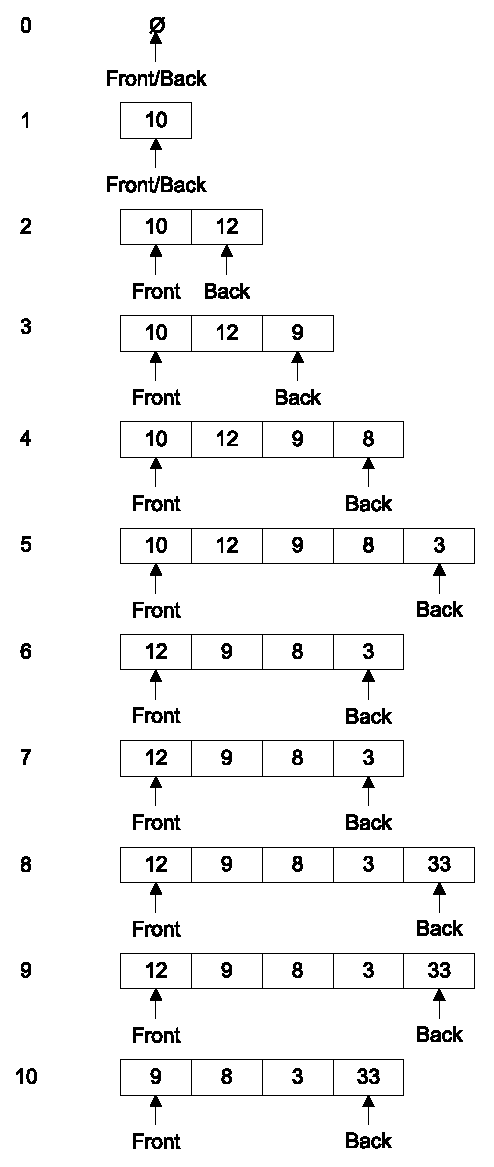
\includegraphics{queue_mutations}
\end{center}
\caption{Queue mutations} \label{fig:queue_mutations}
\end{figure}

\section{Standard Queue}
A queue is implicitly like that described prior to this section, in DSA we don't provide a standard queue because queues are so popular and such a core data structure you will find that pretty much every mainstream library provides a queue data structure that you can use with your language of choice. In this section we will discuss how you can, if required implement an efficient queue data structure.

The main property of a queue is that we have access to the item at the front of the queue, the queue data structure can be efficiently implemented using a singly linked list (defined in \S\ref{singly_linked_list}). A singly linked list provides $O(1)$ insertion, and deletion run time complexities - the reason we have an $O(1)$ run time complexity for deletion is because we only ever in a queue remove the item at the front (Dequeue) and since we always have a pointer to the item at the head of a singly linked list removal is simply a case of returning the value of the old head node, and then modifying the head pointer to be the next node of the old head node. The run time complexity for searching a queue remains the same as that of a singly linked list, $O(n)$.

\section{Priority Queue}
Unlike a standard queue where items are ordered in terms of who arrived first, a priority queue determines the order of its items by using a form of custom comparer to see which item has the highest priority. Other than the items in a priority queue being ordered by priority it remains the same as a normal queue, you can only access the item at the front of the queue.

A sensible implementation of a priority queue is to use a heap data structure (defined in \S\ref{heap}). Using a heap we can look at the first item in the queue by simply returning the item at index $0$ within the heap array. A heap provides us with the ability to construct a priority queue where by the items with the highest priority are either those with the smallest value, or those with the largest.
